\clearpage
\section{The held-out judge}
\label{app:heldout}

The held-out judge (\heldoutjudge) scores every conversation on the same eight instruments and
runs the same utterance coder as the training oracle (\S\ref{sec:setup}); it took no part in
training. Its levels sit $1.2$--$1.8$ points below the training oracle's on \QQ, so only its
contrasts are set beside the body's, never its levels. This appendix collects its version of each
results section: the all-instrument grid (Figure~\ref{fig:grid-heldout}) and the complete score
table (Table~\ref{tab:scores-heldout}) for \S\ref{sec:reward}, the process figure
(Figure~\ref{fig:process-heldout}) for \S\ref{sec:therapist}, and the process table
(Table~\ref{tab:process-heldout}) for \S\ref{sec:patient}.

\textbf{Where it agrees and where it differs.} Across the 21 model states it preserves the sign of
$88.3\%$ of the pairwise state $\times$ instrument contrasts the training oracle makes
(Appendix~\ref{app:saturation}), and it agrees on the direction of every contrast at iteration 10
in the body. On \QQ\ it separates the runs at 7 of the 10 iterations (4--10) where the training
oracle does at 6; its best $\Kz$ checkpoint is iteration 3, which the final $\Kf$ policy still
leads ($\dz\,0.386$), and its gain ratios are $2.50$ against $\Kz$'s last checkpoint and $1.30$
against its best. The one place it favours $\Kz$ is MITI and MICI at iteration 3. On the process
it reads more of the $\Kf$ policy's turns as non-specific praise ($0.20$ at iteration 10, against
the training oracle's $0.05$), so on its reading the $\Kf$ policy's MI-inconsistent share at
iteration 10 is $0.47$, lower than $\Kz$'s $0.80$ but more than double the Base's $0.21$; along the
run it has $\Kz$ lower at iterations 3 and 5 and $\Kf$ lower at 8 and 10. It also sees the $\Kf$
policy persuade after $0.58$ of the patient's sustain talk (Base $0.25$) and reflect sustain talk
more often than $\Kz$ ($0.17$ vs.\ $0.05$), and change-talk persistence separates the runs from
iteration 3 rather than 5.

\begin{table}[t]
\centering
\footnotesize
\setlength{\tabcolsep}{2pt}
\renewcommand{\arraystretch}{0.95}
\begin{tabular}{@{}lrrrl@{}}
\toprule
Per-conversation measure & Base & $\Kz$ & $\Kf$ & \dz\\
\midrule
\multicolumn{5}{@{}l}{\emph{Therapist turns (share by dominant function)}}\\
non-specific praise ($\downarrow$) & $0.038$ & $0.762$ & $\mathbf{0.203}$ & $-2.19^{***}$\\
complex reflection & $0.031$ & $0.016$ & $\mathbf{0.242}$ & $+0.94^{***}$\\
persuasion ($\downarrow$) & $0.166$ & $\mathbf{0.033}$ & $0.268$ & $+0.83^{***}$\\
MI-adherent share & $0.283$ & $0.037$ & $\mathbf{0.360}$ & $+1.35^{***}$\\
MI-inconsistent share ($\downarrow$) & $0.214$ & $0.795$ & $\mathbf{0.471}$ & $-1.08^{***}$\\
\midrule
\multicolumn{5}{@{}l}{\emph{The therapist's reply to the patient's \ldots}}\\
change talk: reflects it & $0.030$ & $0.006$ & $\mathbf{0.258}$ & $+0.99^{***}$\\
sustain talk: praises ($\downarrow$) & $0.011$ & $0.723$ & $\mathbf{0.011}$ & $-3.10^{***}$\\
sustain talk: persuades ($\downarrow$) & $0.253$ & $\mathbf{0.056}$ & $0.580$ & $+1.61^{***}$\\
sustain talk: reflects it & $0.081$ & $0.050$ & $\mathbf{0.171}$ & $+0.49^{**}$\\
\midrule
\multicolumn{5}{@{}l}{\emph{Next patient utterance is change talk, after \ldots}}\\
change talk & $0.715$ & $0.734$ & $\mathbf{0.935}$ & $+0.65^{***}$\\
sustain talk & $0.182$ & $0.193$ & $0.238$ & $+0.04$\\
\midrule
\multicolumn{5}{@{}l}{\emph{The session}}\\
change-talk share & $0.463$ & $0.545$ & $\mathbf{0.721}$ & $+0.70^{***}$\\
\bottomrule
\end{tabular}
\caption{Table~\ref{tab:process} under the held-out judge (iteration 10; same columns, conventions
and tests). Its paired contrasts that start from a patient utterance use $64$--$80$ personas.}
\label{tab:process-heldout}
\end{table}

\begin{figure*}[t]
\centering
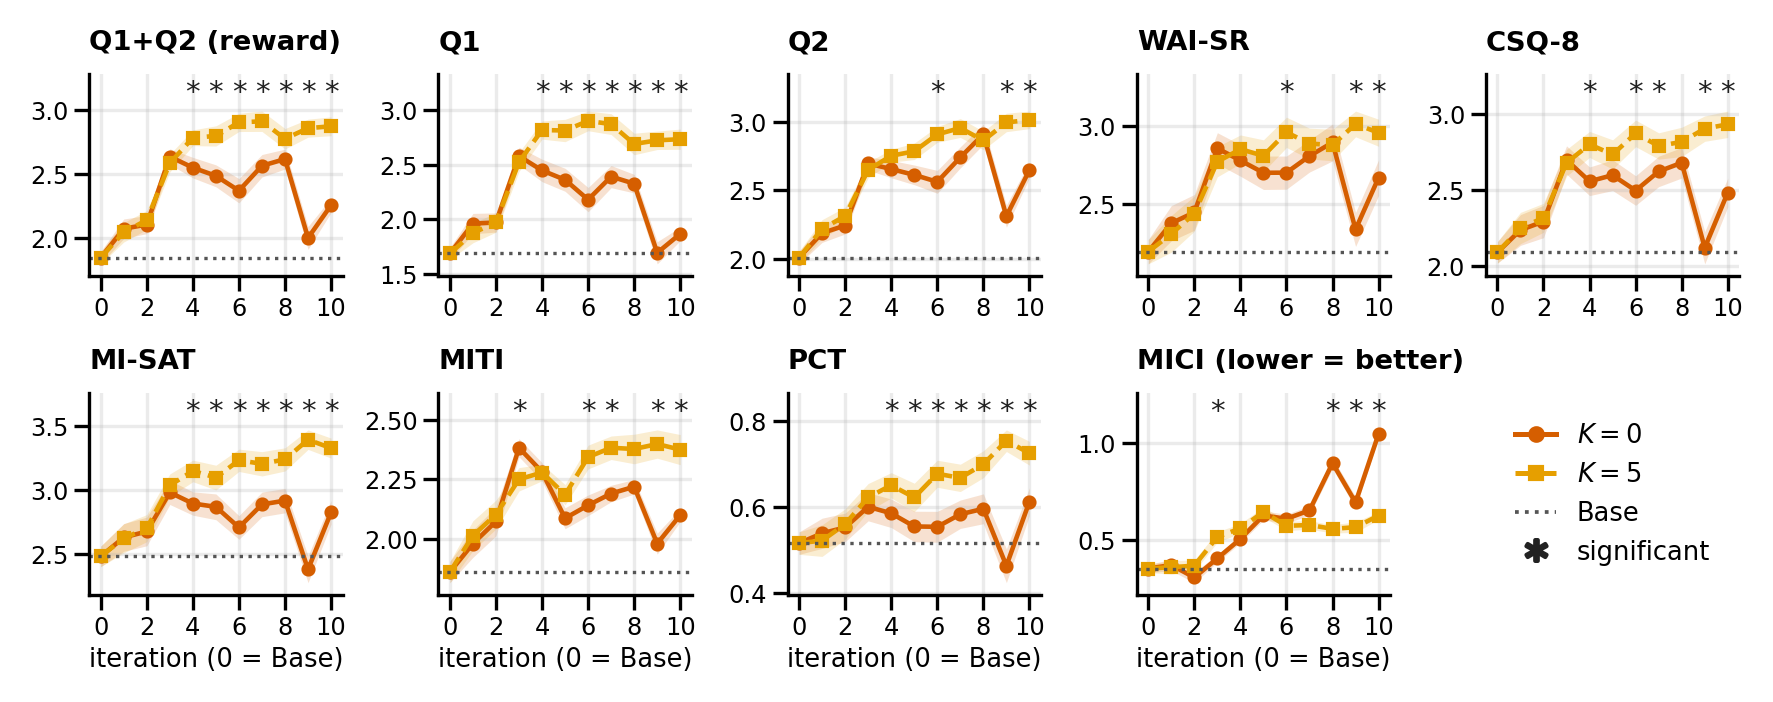
\includegraphics[width=0.94\textwidth]{figures/levels_grid_grpo_claude-haiku-4-5.png}
\caption{Figure~\ref{fig:headline} under the held-out judge: every instrument by iteration, mean
$\pm$ SE over the 96 personas, from the Base (dotted line); a star marks a significant $\Kf$ vs.\
$\Kz$ contrast, which at iteration 3 favours $\Kz$ on MITI and MICI. Levels are in this judge's own
units and are not comparable to Figure~\ref{fig:headline}'s.}
\label{fig:grid-heldout}
\end{figure*}

\begin{table*}[t]
\centering
\footnotesize
\setlength{\tabcolsep}{4.5pt}
\renewcommand{\arraystretch}{0.92}
\begin{tabular}{@{}lrrrrrrrrr@{}}
\toprule
Iteration & \QQ & Q1 & Q2 & WAI-SR & CSQ-8 & MI-SAT & MITI & PCT & MICI ($\downarrow$)\\
\midrule
Base & $1.848$ & $1.688$ & $2.008$ & $2.194$ & $2.089$ & $2.480$ & $1.859$ & $0.516$ & $0.355$\\
\midrule
\multicolumn{10}{@{}l}{\emph{$K{=}0$}}\\
1 & $2.074$ & $1.960$ & $2.188$ & $2.377$ & $2.237$ & $2.628$ & $1.979$ & $0.539$ & $0.373$\\
2 & $2.107$ & $1.971$ & $2.243$ & $2.446$ & $2.293$ & $2.675$ & $2.073$ & $0.553$ & $0.309$\\
3 & $2.637$ & $2.577$ & $2.696$ & $2.858$ & $2.699$ & $2.981$ & $2.383$\rlap{$^{*}$} & $0.601$ & $0.407$\rlap{$^{*}$}\\
4 & $2.550$ & $2.446$ & $2.655$ & $2.780$ & $2.559$ & $2.894$ & $2.281$ & $0.586$ & $0.508$\\
5 & $2.487$ & $2.360$ & $2.613$ & $2.701$ & $2.599$ & $2.868$ & $2.086$ & $0.555$ & $0.629$\\
6 & $2.371$ & $2.179$ & $2.562$ & $2.701$ & $2.497$ & $2.707$ & $2.141$ & $0.554$ & $0.612$\\
7 & $2.565$ & $2.390$ & $2.741$ & $2.808$ & $2.624$ & $2.887$ & $2.190$ & $0.583$ & $0.655$\\
8 & $2.617$ & $2.325$ & $2.909$ & $2.895$ & $2.681$ & $2.917$ & $2.219$ & $0.596$ & $0.898$\\
9 & $2.002$ & $1.694$ & $2.311$ & $2.337$ & $2.120$ & $2.378$ & $1.979$ & $0.463$ & $0.696$\\
10 & $2.257$ & $1.867$ & $2.648$ & $2.669$ & $2.484$ & $2.825$ & $2.099$ & $0.612$ & $1.050$\\
\midrule
\multicolumn{10}{@{}l}{\emph{$K{=}5$}}\\
1 & $2.046$ & $1.875$ & $2.218$ & $2.308$ & $2.250$ & $2.622$ & $2.013$ & $0.522$ & $0.362$\\
2 & $2.142$ & $1.971$ & $2.312$ & $2.438$ & $2.318$ & $2.701$ & $2.102$ & $0.560$ & $0.370$\\
3 & $2.586$ & $2.523$ & $2.649$ & $2.772$ & $2.681$ & $3.036$ & $2.250$ & $0.623$ & $0.518$\\
4 & $2.784$\rlap{$^{*}$} & $2.815$\rlap{$^{*}$} & $2.752$ & $2.852$ & $2.802$\rlap{$^{*}$} & $3.149$\rlap{$^{*}$} & $2.279$ & $0.651$\rlap{$^{*}$} & $0.562$\\
5 & $2.798$\rlap{$^{*}$} & $2.810$\rlap{$^{*}$} & $2.785$ & $2.810$ & $2.736$ & $3.097$\rlap{$^{*}$} & $2.185$ & $0.622$\rlap{$^{*}$} & $0.647$\\
6 & $2.903$\rlap{$^{*}$} & $2.898$\rlap{$^{*}$} & $2.909$\rlap{$^{*}$} & $2.960$\rlap{$^{*}$} & $2.875$\rlap{$^{*}$} & $3.233$\rlap{$^{*}$} & $2.344$\rlap{$^{*}$} & $0.677$\rlap{$^{*}$} & $0.575$\\
7 & $2.912$\rlap{$^{*}$} & $2.869$\rlap{$^{*}$} & $2.955$ & $2.888$ & $2.792$\rlap{$^{*}$} & $3.205$\rlap{$^{*}$} & $2.383$\rlap{$^{*}$} & $0.668$\rlap{$^{*}$} & $0.580$\\
8 & $2.776$\rlap{$^{*}$} & $2.688$\rlap{$^{*}$} & $2.864$ & $2.878$ & $2.819$ & $3.240$\rlap{$^{*}$} & $2.378$ & $0.700$\rlap{$^{*}$} & $0.560$\rlap{$^{*}$}\\
9 & $2.858$\rlap{$^{*}$} & $2.721$\rlap{$^{*}$} & $2.996$\rlap{$^{*}$} & $3.014$\rlap{$^{*}$} & $2.906$\rlap{$^{*}$} & $3.394$\rlap{$^{*}$} & $2.398$\rlap{$^{*}$} & $0.754$\rlap{$^{*}$} & $0.568$\rlap{$^{*}$}\\
10 & $2.873$\rlap{$^{*}$} & $2.731$\rlap{$^{*}$} & $3.015$\rlap{$^{*}$} & $2.957$\rlap{$^{*}$} & $2.935$\rlap{$^{*}$} & $3.328$\rlap{$^{*}$} & $2.375$\rlap{$^{*}$} & $0.725$\rlap{$^{*}$} & $0.628$\rlap{$^{*}$}\\
\bottomrule
\end{tabular}
\caption{Table~\ref{tab:scores} under the held-out judge: every instrument at every iteration, the
mean over the 96 personas (the Base: over its 192 conversations), a star on the better run where
the $\Kf$ vs.\ $\Kz$ contrast is significant (Holm across iterations 1--10 within instrument). The
two stars on $\Kz$ cells are MITI and MICI at iteration 3. Levels are in this judge's own units.}
\label{tab:scores-heldout}
\end{table*}

\begin{figure*}[t]
\centering
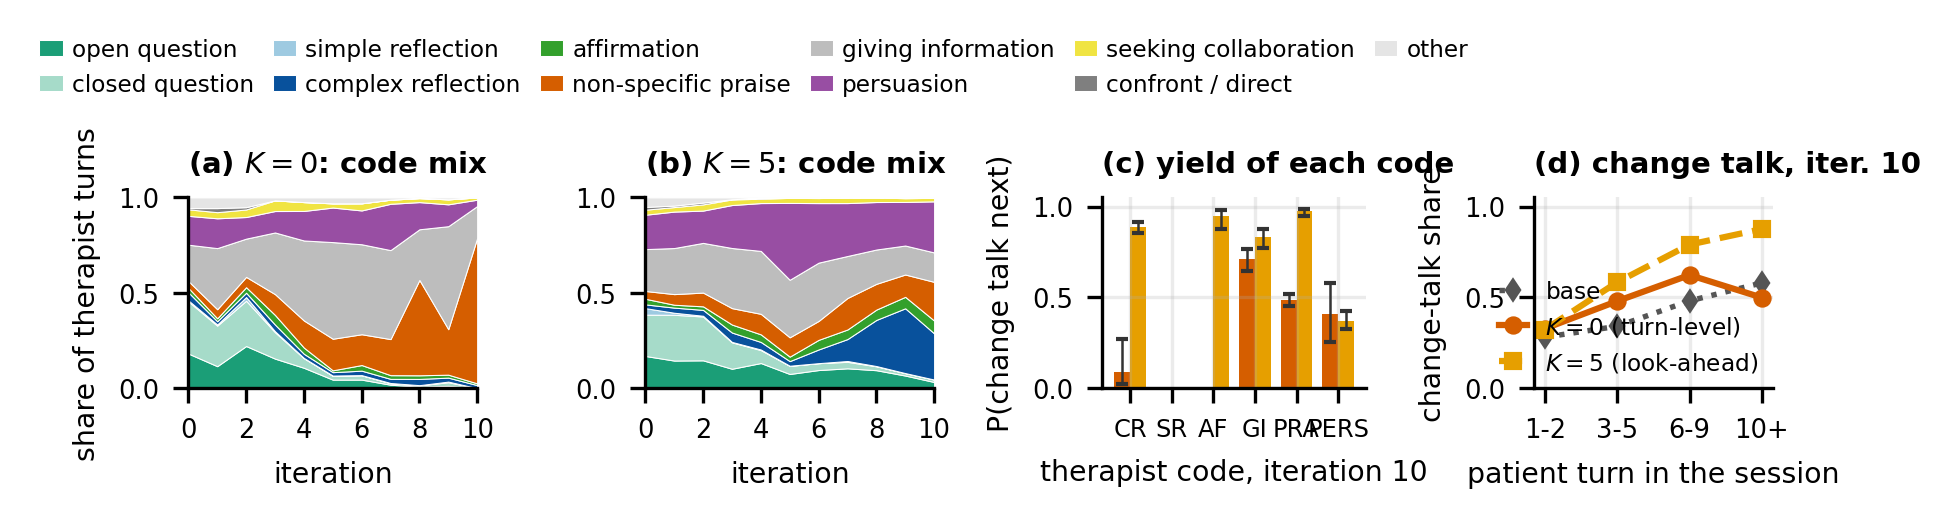
\includegraphics[width=0.94\textwidth]{figures/process_grpo_heldout.png}
\caption{Figure~\ref{fig:process} under the held-out judge: \textbf{(a, b)} each run's code mix
by iteration, \textbf{(c)} change-talk persistence by iteration (mean $\pm$ SE over conversations;
dotted: the Base), \textbf{(d)} the change-talk share of patient utterances by position in the
session at iteration 10 against the Base. The held-out judge reads more of the $\Kf$ policy's
turns as non-specific praise than the training oracle does ($0.20$ vs.\ $0.05$ at iteration 10)
and agrees on the direction of everything else in the picture.}
\label{fig:process-heldout}
\end{figure*}

